\PID
%
\begin{figure}[b!]
    \centering
    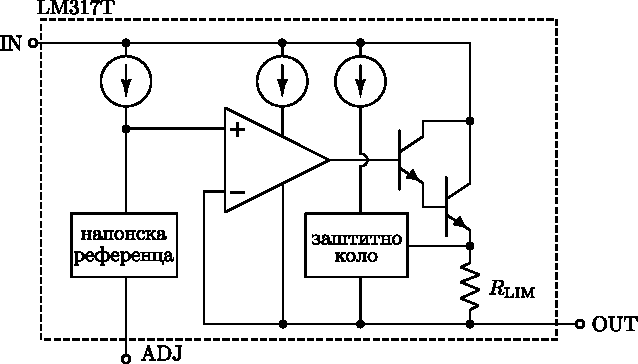
\includegraphics[scale=1]{fig/LM317T.pdf}
    \caption{}
    \label{fig:\ID:LM317}
\end{figure}
%
На слици је приказана принципска шема LM317T интегрисаног подесивог регулатора. Напон напонске 
референце је $V_{\rm R} = 1,25\unit{V}$. Струјна заштита је са константном струјом која 
износи $I_{\rm max} = 1,5\unit{A}$, док су термичка отпорности спој-амбијент и спој-кућиште 
$R_{\rm \uptheta JA} = 80\unit{^\circ C/W}$ и 
$R_{\rm \uptheta JC} = 5\unit{^\circ C/W}$, респективно. 
а максимална радна температура је $T_{\rm max} = 125\unit{^\circ C}$. Температура амбијента је
 $T_{\rm A} = 25\unit{^\circ C}$, а расположива је једна батерија за напајање $V_{\rm CC} = 12\unit{V}$.


\begin{enumerate}[label=(\alph*)]
\item Уцртати безбедну област рада овог стабилизатора у дијаграму излазног напона и струје. 
\item Пројектовати стабилизатор напона номиналне вредности 
$V_{\rm I} = 5\unit{V}$, и израчунати максималну безбедну струју оптерећења на излазу стабилизатора.
\item Уколико се стабилизатору дода хладњак чија је термичка отпорност 
$R_{\rm \uptheta JA} = 20\unit{^\circ C/W}$, одредити колико се повећава максимална безбедна снага потрошње стабилизатора.
\end{enumerate}
\REZULTAT
